\subsection{Piece-wise Functions}
\begin{definition}[Piece-wise Functions]
	A single function that uses two or more different formulas or rules, with each rule applying to a specific portion of the function's domain.
\end{definition}

\begin{example}[Algebraic]
	\hfill
	\begin{enumerate}
		\item $$f(x) = \begin{cases}
		 	   x^3 & \text{if } x < 1 \\
			   3x - 2 & \text{if } x \ge 1
			\end{cases}$$
		\begin{enumerate}
			\item $f(-1) = (-1)^3 \to (-1, -1)$
			\item $f(0) = (0)^3 \to (0, 0)$
			\item $f(1) = 3(1) - 2 \to (1, 1)$
		\end{enumerate}
		\item $$f(x) = \begin{cases}
			   x^2 & \text{if } x < 0 \\
			   2 & \text{if } x = 0 \\
			   2x + 1 & \text{if } x > 0
			\end{cases}$$
		\begin{enumerate}
			\item $f(-2) = (-2)^2 \to (-2, 4)$
			\item $f(0) = 2 \to (0, 2)$
			\item $f(2) = 2(2) + 1 \to (2, 5)$
		\end{enumerate}
	\end{enumerate}
\end{example}

\begin{example}[Graph] 
	\hfill
	\begin{enumerate}
		\item $$f(x) = \begin{cases}
		  x^3 & \text{if } x < 1 \\
		  3x - 2 & \text{if } x \ge 1
		\end{cases}$$
		\begin{center}
		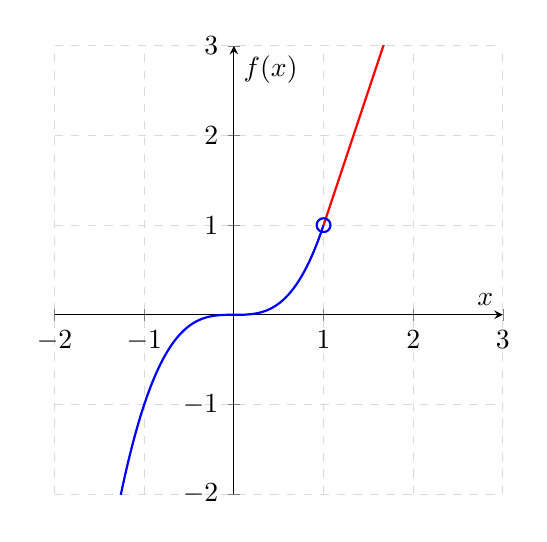
\begin{tikzpicture}
			\begin{axis}[
			    axis lines = center,
			    xlabel = $x$,
			    ylabel = $f(x)$,
			    xmin = -2, xmax = 3,
			    ymin = -2, ymax = 3,
			    grid = major,
			    grid style = {dashed, gray!30},
			    axis equal image
			]
			    \addplot [domain=-2:1, samples=100, thick, blue] {x^3};
				\addplot [domain=1:2.6, samples=100, thick, red] {3*x - 2};
				\draw[blue, thick] (axis cs:1,1) circle (2.5pt);
			\end{axis}
		\end{tikzpicture}
		\end{center}
		\item $$f(x) = \begin{cases}
			   x^2 & \text{if } x < 0 \\
			   2 & \text{if } x = 0 \\
			   2x + 1 & \text{if } x > 0
			\end{cases}$$
		\begin{center}
		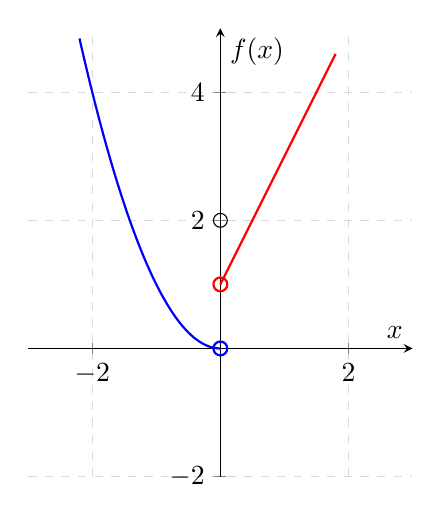
\begin{tikzpicture}
			\begin{axis}[
			    axis lines = center,
			    xlabel = $x$,
			    ylabel = $f(x)$,
			    xmin = -3, xmax = 3,
			    ymin = -2, ymax = 5,
			    grid = major,
			    grid style = {dashed, gray!30},
			    axis equal image
			]
			    \addplot [domain=-2.2:0, samples=100, thick, blue] {x^2};
				\addplot [domain=0:1.8, samples=100, thick, red] {2*x + 1};
				\draw[blue, thick] (axis cs:0,0) circle (2.5pt);
				\draw[red, thick] (axis cs:0,1) circle (2.5pt);
				\draw[black] (axis cs:0,2) circle (2.5pt);
			\end{axis}
		\end{tikzpicture}
		\end{center}
	\end{enumerate}
\end{example}

\begin{definition}[Not Continuous Function]
	In a piece-wise function, a function is not continuous \textit{(discontinuous)} at a point if the different sub-functions do not connect seamlessly at the transition boundary
\end{definition}

\begin{example}[Not Continouous Function]
	$$f(x) = \begin{cases}
	  x + 3 & \text{if } -4 \le x < -2 \\
	  -2x - 3 & \text{if } x > -2
	\end{cases}$$
	\begin{example}[Graph] 
		\hfill
		\begin{center}
		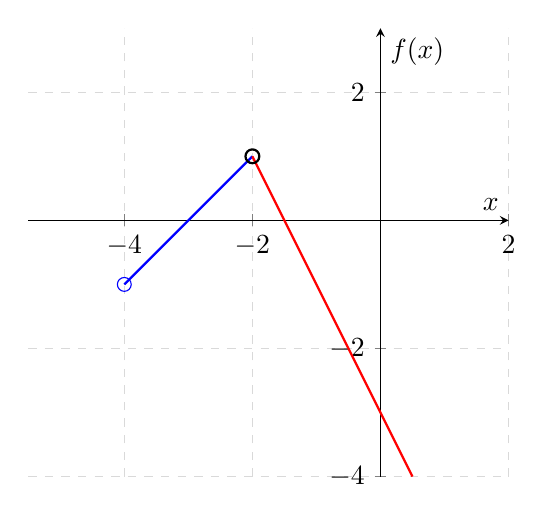
\begin{tikzpicture}
			\begin{axis}[
			    axis lines = center,
			    xlabel = $x$,
			    ylabel = $f(x)$,
			    xmin = -5.5, xmax = 2,
			    ymin = -4, ymax = 3,
			    grid = major,
			    grid style = {dashed, gray!30},
			    axis equal image 
			]
			    \addplot [domain=-4:-2, samples=100, thick, blue] {x + 3};
				\addplot [domain=-2:0.5, samples=100, thick, red] {-2*x - 3};
				\draw[blue] (axis cs:-4,-1) circle (2.5pt);
				\draw[black, thick] (axis cs:-2,1) circle (2.5pt);	
			\end{axis}
		\end{tikzpicture}
		\end{center}
	\end{example}
\end{example}
